\documentclass[aspectratio=169,11pt]{beamer}

\usepackage[utf8]{inputenc}
\usepackage[T1]{fontenc}
\usepackage{lmodern}
\usepackage[provide=*]{babel}
\babelprovide[import,main]{french}
\usepackage{graphicx}
\usepackage{hyperref}
\usepackage{amsmath}

\usetheme{Madrid}
\setbeamertemplate{navigation symbols}{}

\title{Projet 1 -- Plateforme de priorisation des vulnerabilites IoT}
\subtitle{8INF917 -- Securite informatique pour l'Internet des Objets}
\author{A. Bidet \and C. Bellenge \and J. Balsan \and M. Fousset}
\institute{Universite du Quebec a Chicoutimi}
\date{9 mars 2026}

\begin{document}

\begin{frame}
  \titlepage
\end{frame}

\begin{frame}{Plan de la presentation}
\begin{itemize}
  \item Contexte, probleme et objectifs
  \item Architecture et pipeline de collecte
  \item Modele de donnees et methode de priorisation
  \item Fonctionnalites, resultats et limites
  \item Demonstration, conclusion et perspectives
\end{itemize}
\end{frame}

\begin{frame}{Contexte et probleme}
\begin{itemize}
  \item Les objets IoT augmentent vite, les CVE aussi.
  \item Les equipes doivent prioriser avec peu de temps.
  \item CVSS seul ne suffit pas pour decider.
  \item Besoin: passer d'une liste de CVE a un plan d'action.
\end{itemize}
\end{frame}

\begin{frame}{Objectif et perimetre}
\begin{itemize}
  \item Construire une plateforme web defensive de priorisation.
  \item Collecter des donnees open-source automatiquement.
  \item Enrichir avec CVSS, KEV, EPSS et CWE.
  \item Perimetre: cameras IP (domestique/PME).
  \item Aucune action offensive ni scan Internet.
\end{itemize}
\end{frame}

\begin{frame}{Architecture globale}
\begin{columns}[T,onlytextwidth]
  \begin{column}{0.43\textwidth}
    \begin{itemize}
      \item 3 blocs: Next.js, Python, PostgreSQL.
      \item Sources externes: NVD, KEV, EPSS, CWE.
      \item Architecture modulaire et reproductible.
    \end{itemize}
  \end{column}
  \begin{column}{0.57\textwidth}
    \centering
    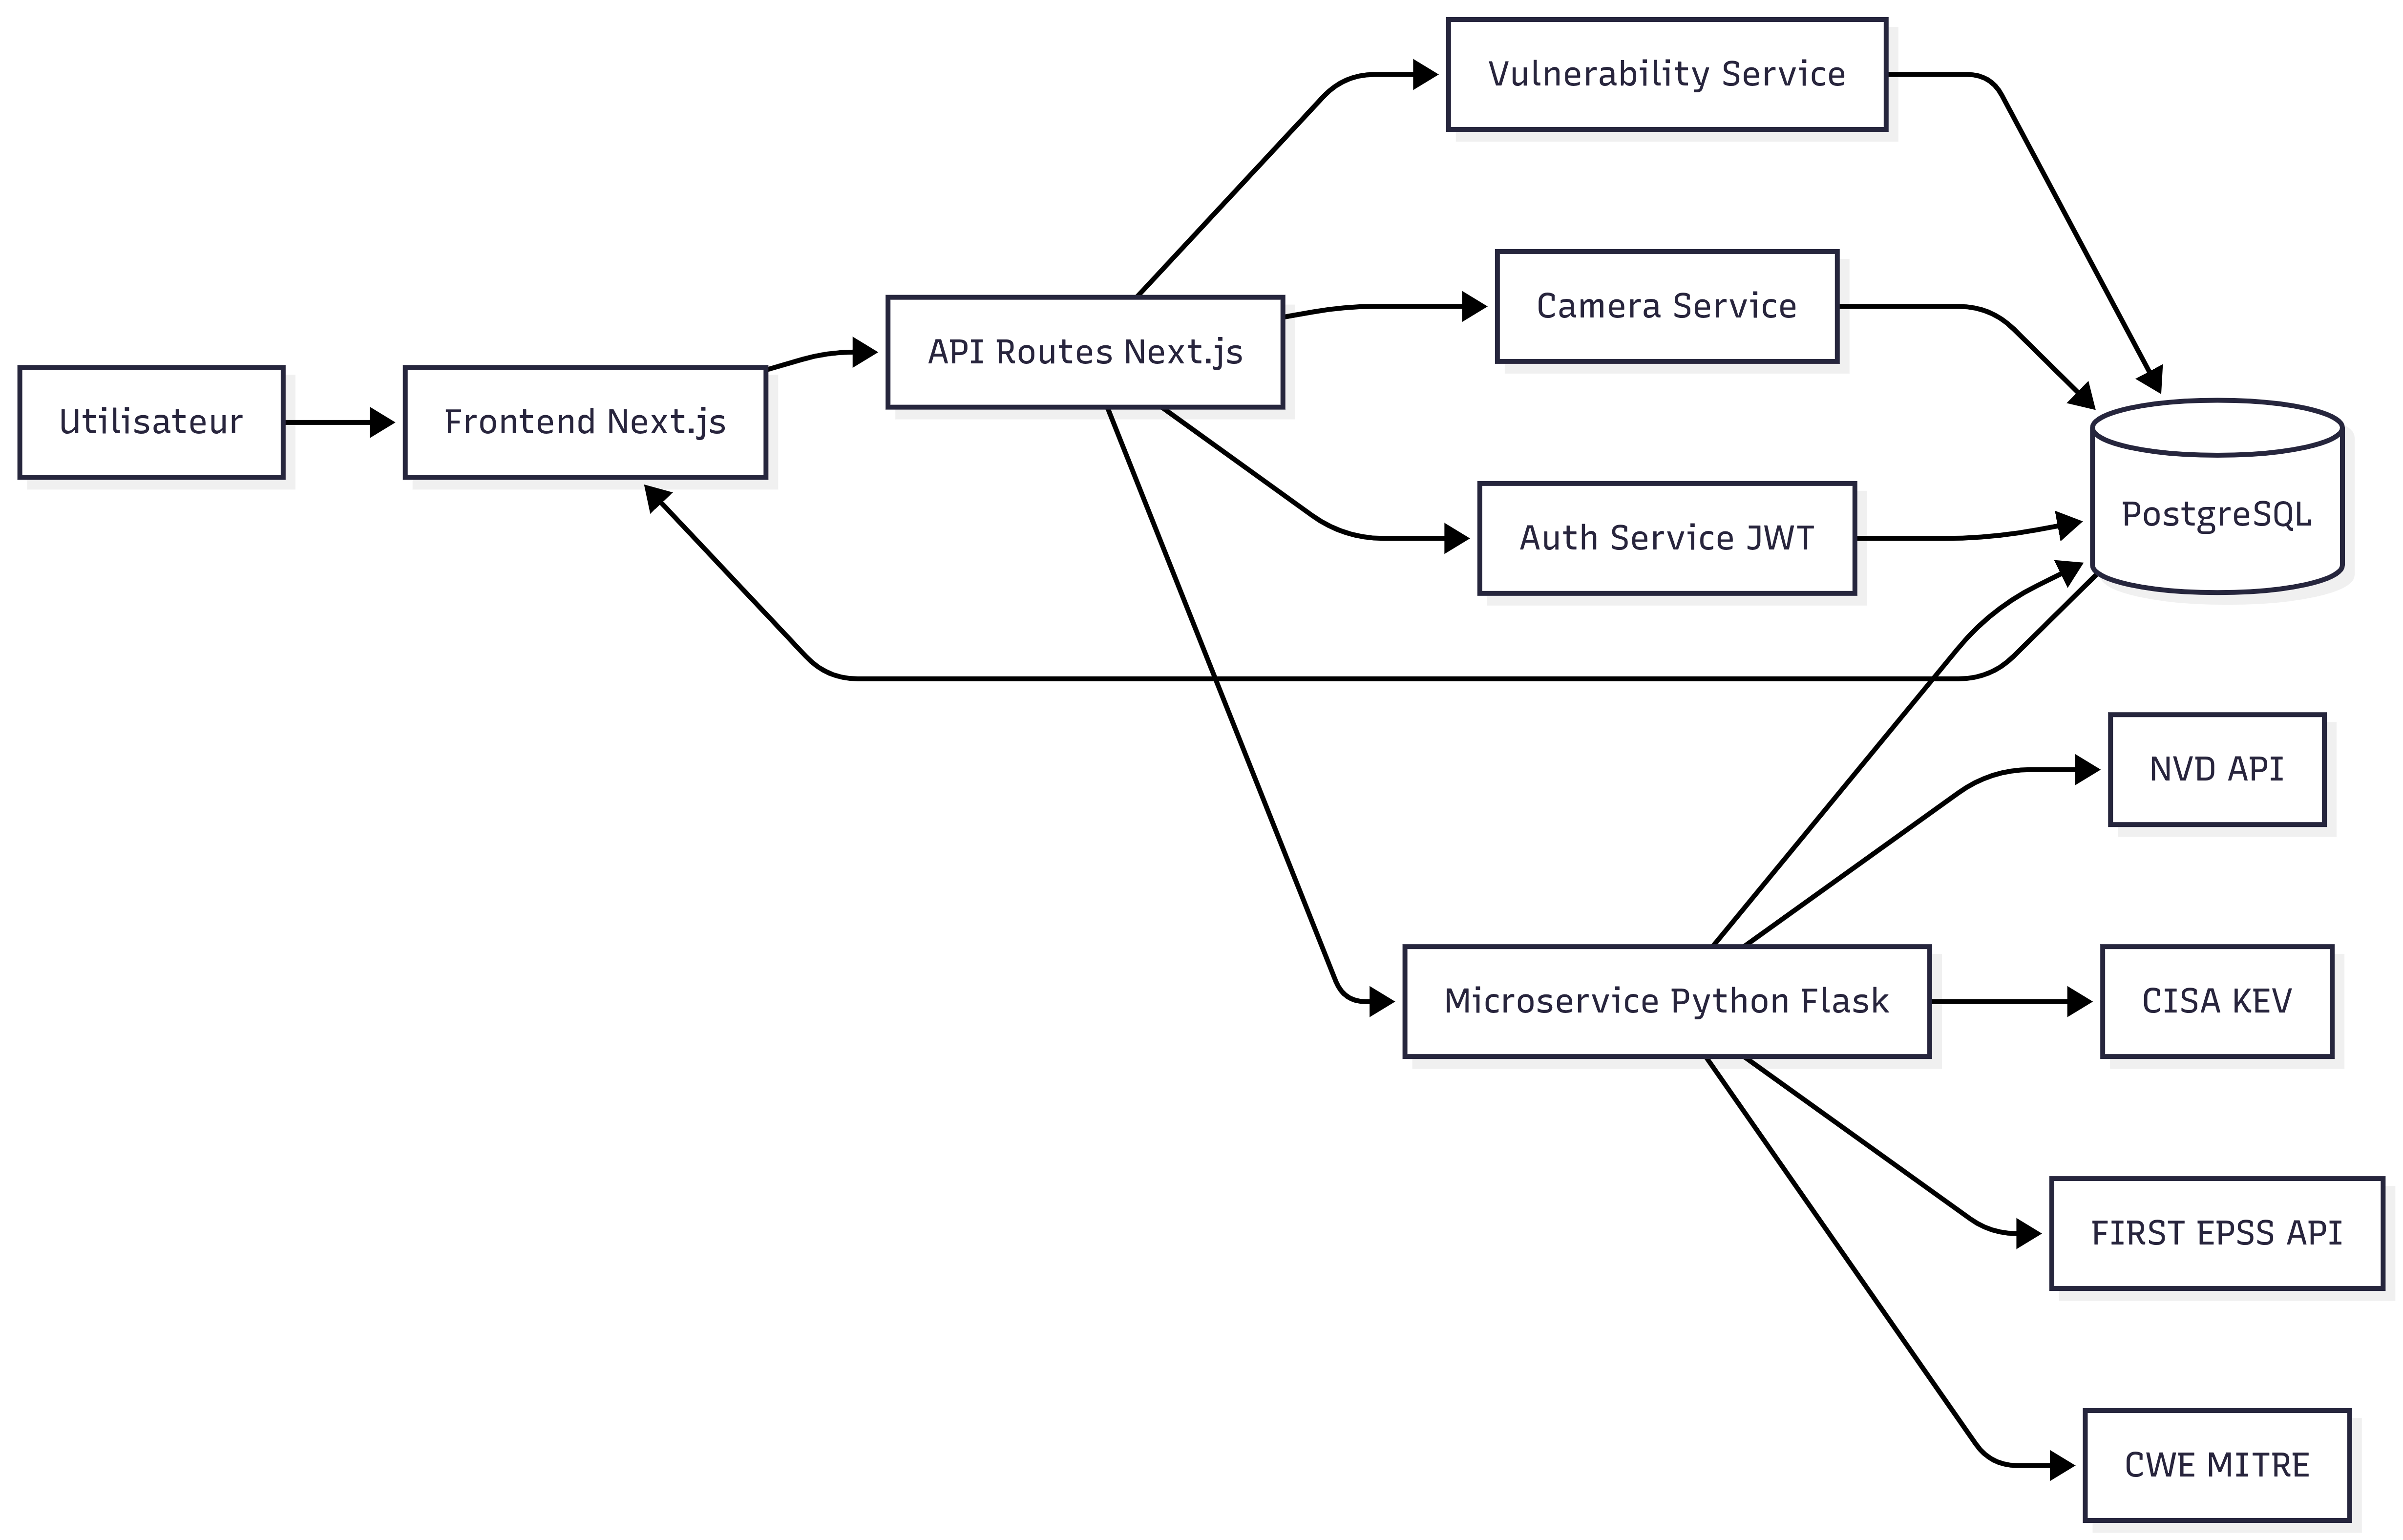
\includegraphics[width=\textwidth,height=0.72\textheight,keepaspectratio]{img/fig01-architecture-globale.png}
  \end{column}
\end{columns}
\end{frame}

\begin{frame}{Pipeline de collecte et enrichissement}
\begin{columns}[T,onlytextwidth]
  \begin{column}{0.43\textwidth}
    \begin{itemize}
      \item Collecte CVE puis normalisation.
      \item Association aux cameras du parc.
      \item Enrichissement KEV/EPSS/CWE.
      \item Publication des indicateurs dans l'UI.
    \end{itemize}
  \end{column}
  \begin{column}{0.57\textwidth}
    \centering
    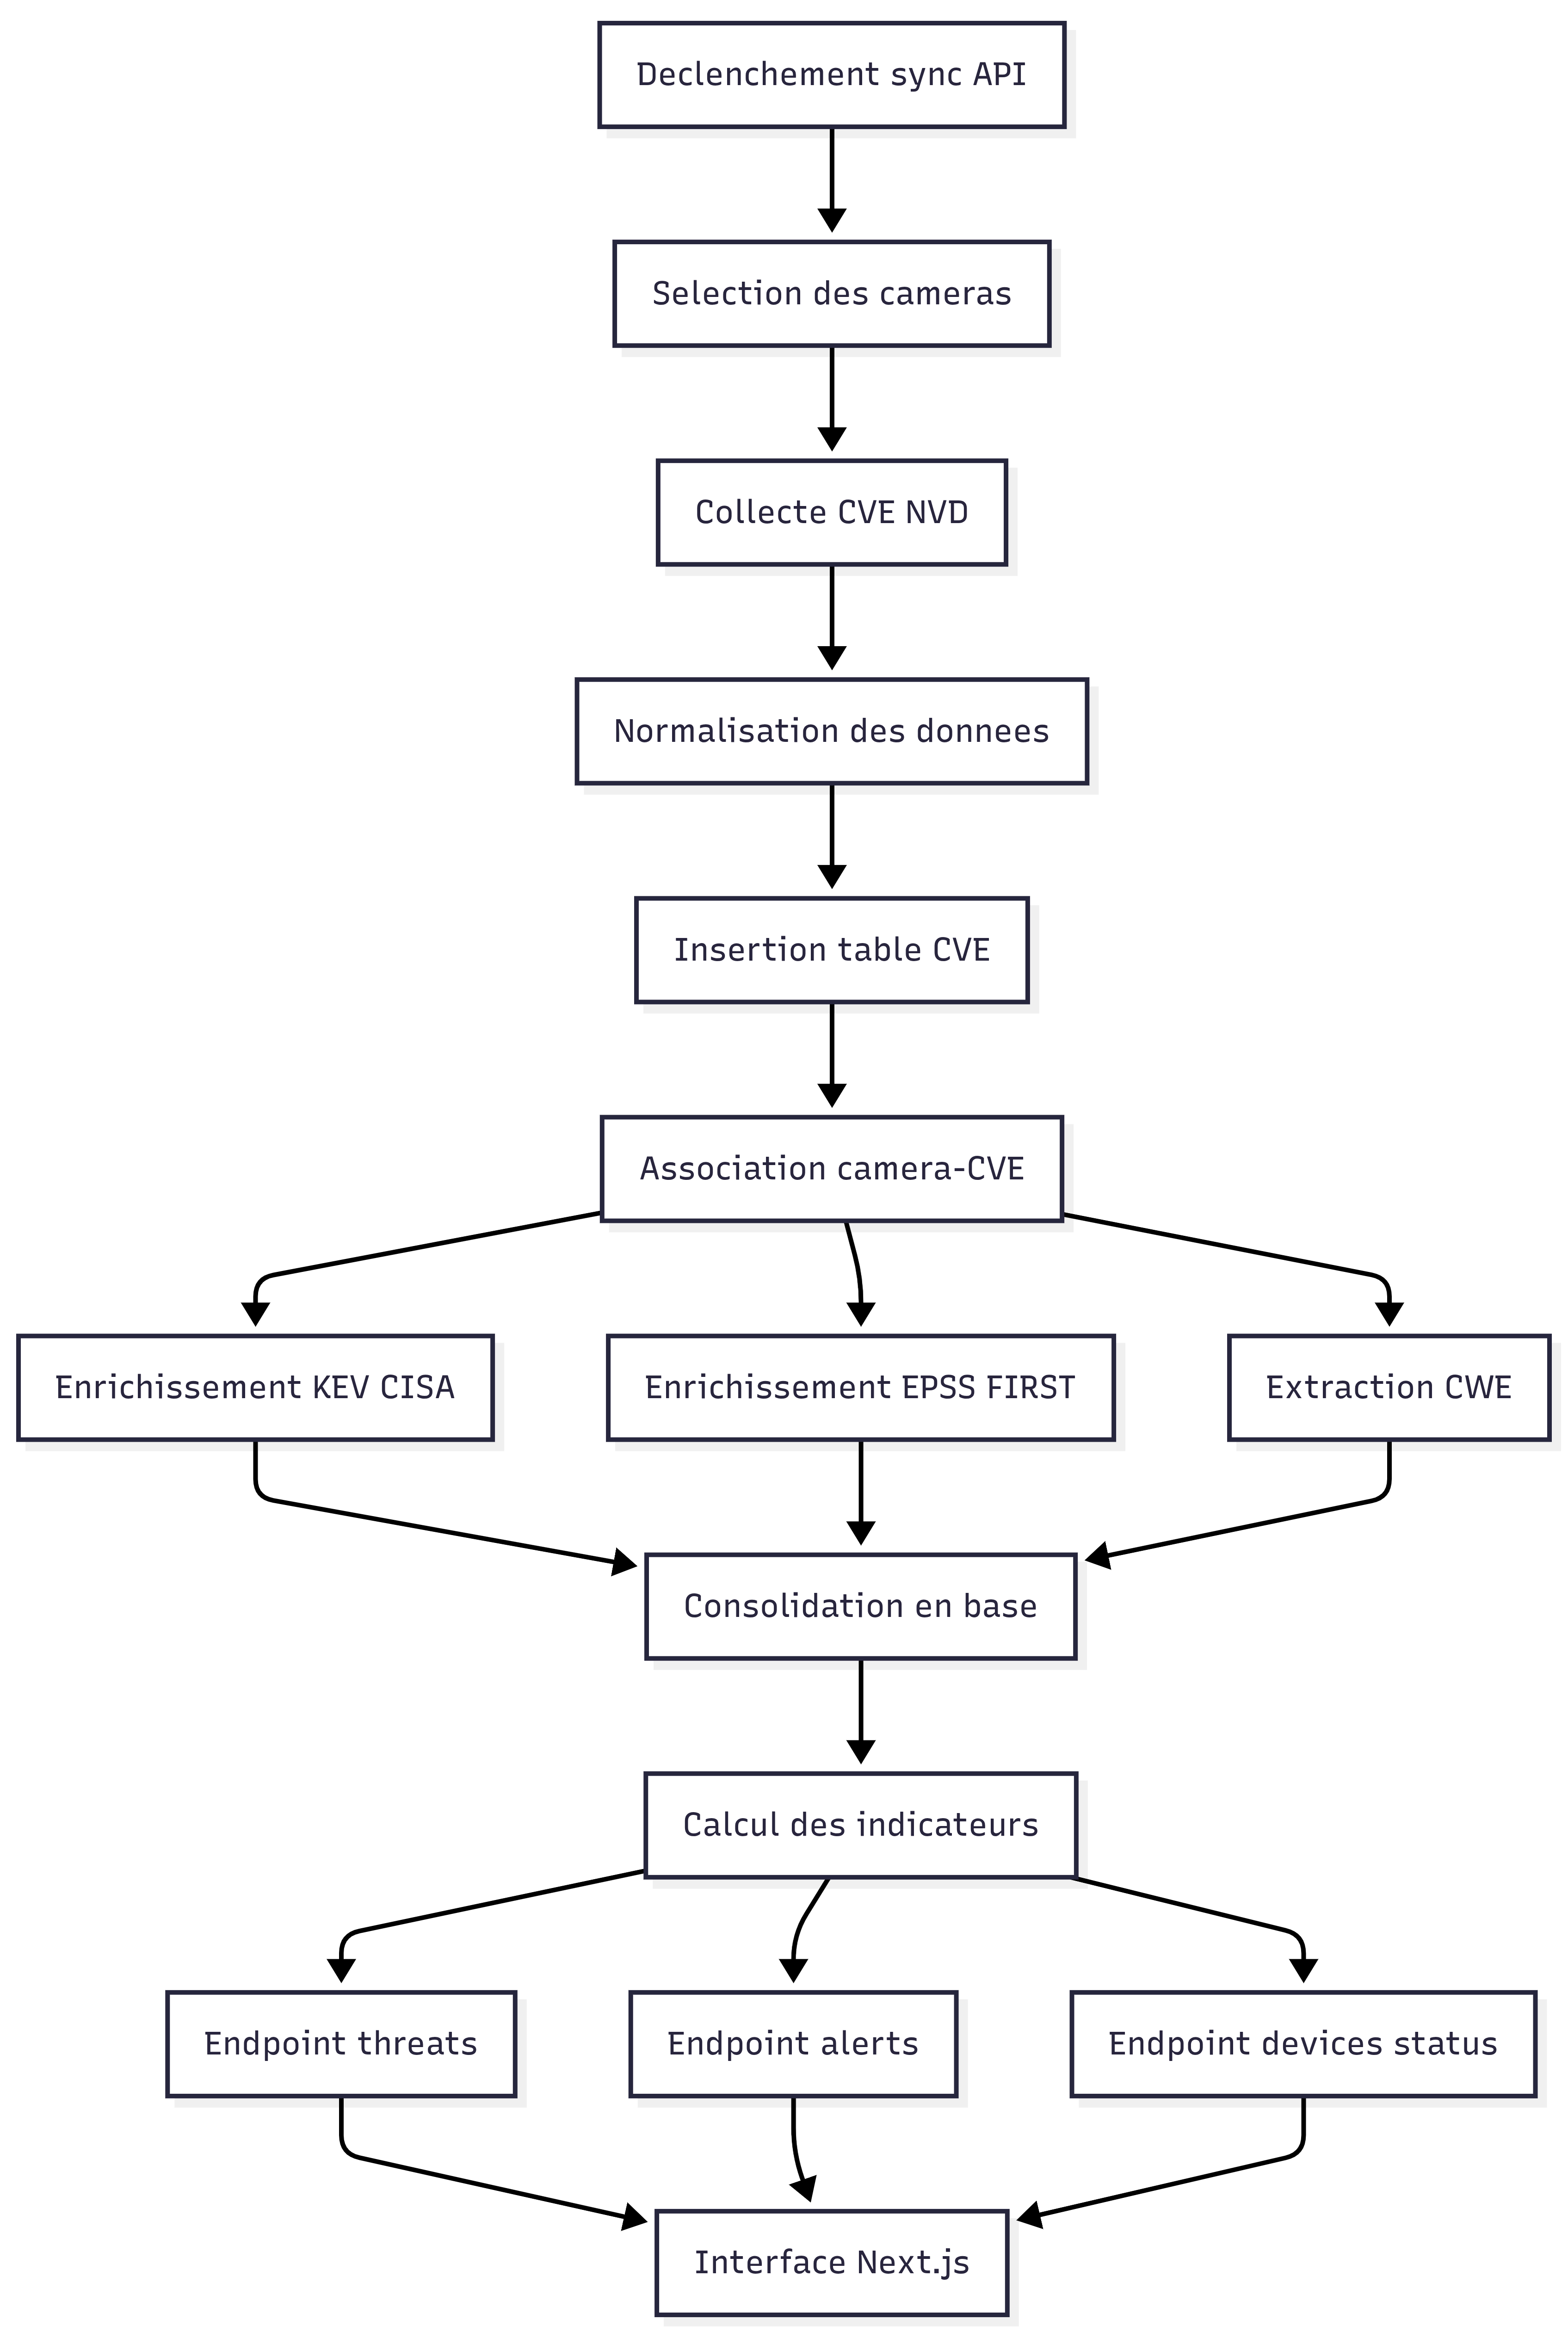
\includegraphics[width=\textwidth,height=0.72\textheight,keepaspectratio]{img/fig02-pipeline-collecte-enrichissement.png}
  \end{column}
\end{columns}
\end{frame}

\begin{frame}{Modele de donnees}
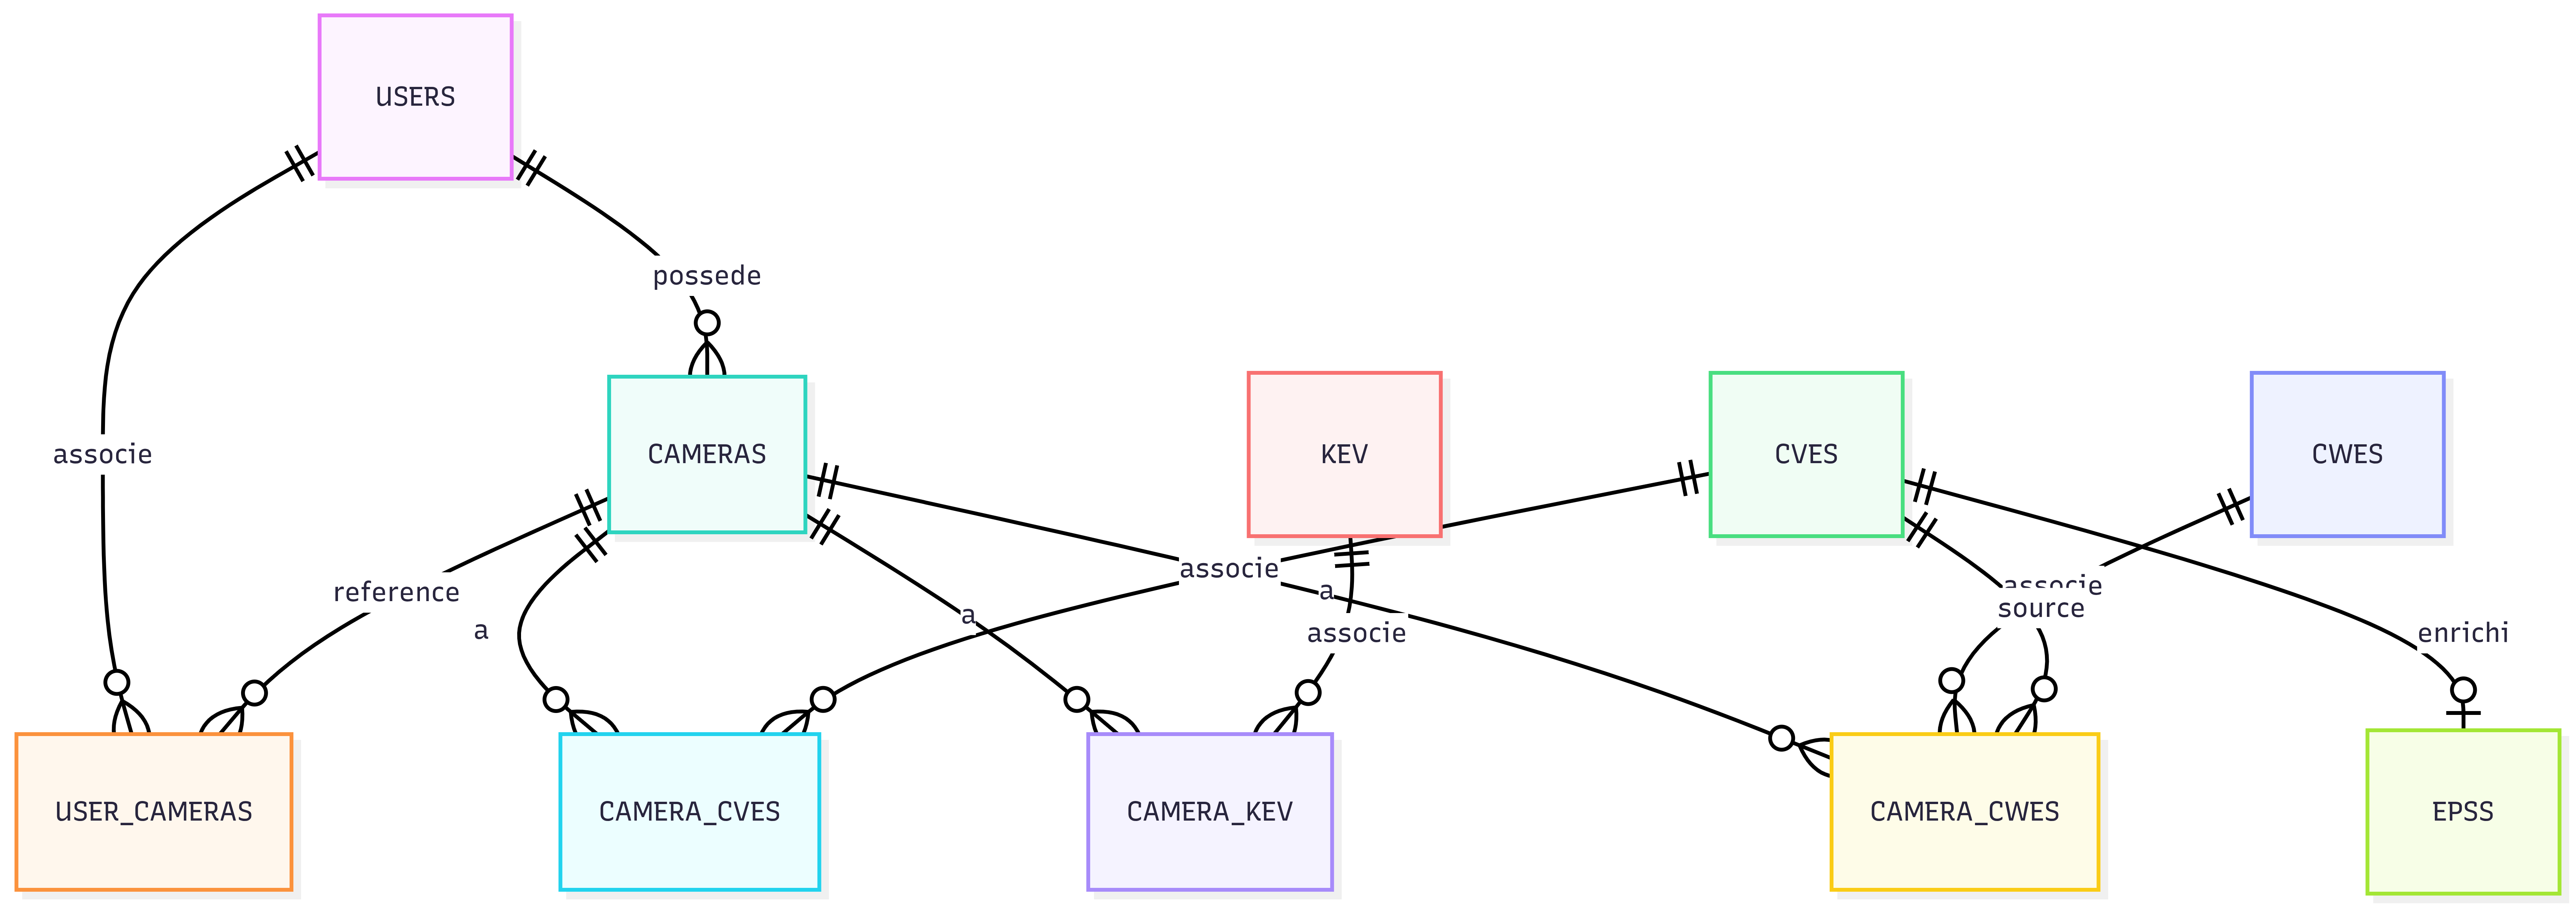
\includegraphics[width=0.95\textwidth,height=0.72\textheight,keepaspectratio]{img/fig03-modele-donnees-relationnel.png}

\vspace{0.4em}
\begin{itemize}
  \item Separation referentiels globaux vs associations camera.
  \item Moins de redondance et requetes plus simples.
  \item Integrite via PK/FK et tables de liaison.
\end{itemize}
\end{frame}

\begin{frame}{Methode de priorisation du risque}
\begin{columns}[T,onlytextwidth]
  \begin{column}{0.43\textwidth}
    \begin{itemize}
      \item Le score CVE combine impact, probabilite et exploitation observee.
      \item Le score appareil agrege les risques les plus critiques.
      \item Objectif: prioriser les corrections a court terme.
    \end{itemize}
    \vspace{0.3em}
    {\scriptsize
    \[
    \text{Risk}_{CVE} = 100 \times \left(0.6\times\frac{CVSS}{10} + 0.3\times EPSS + 0.1\times KEV\right)
    \]
    }
  \end{column}
  \begin{column}{0.57\textwidth}
    \centering
    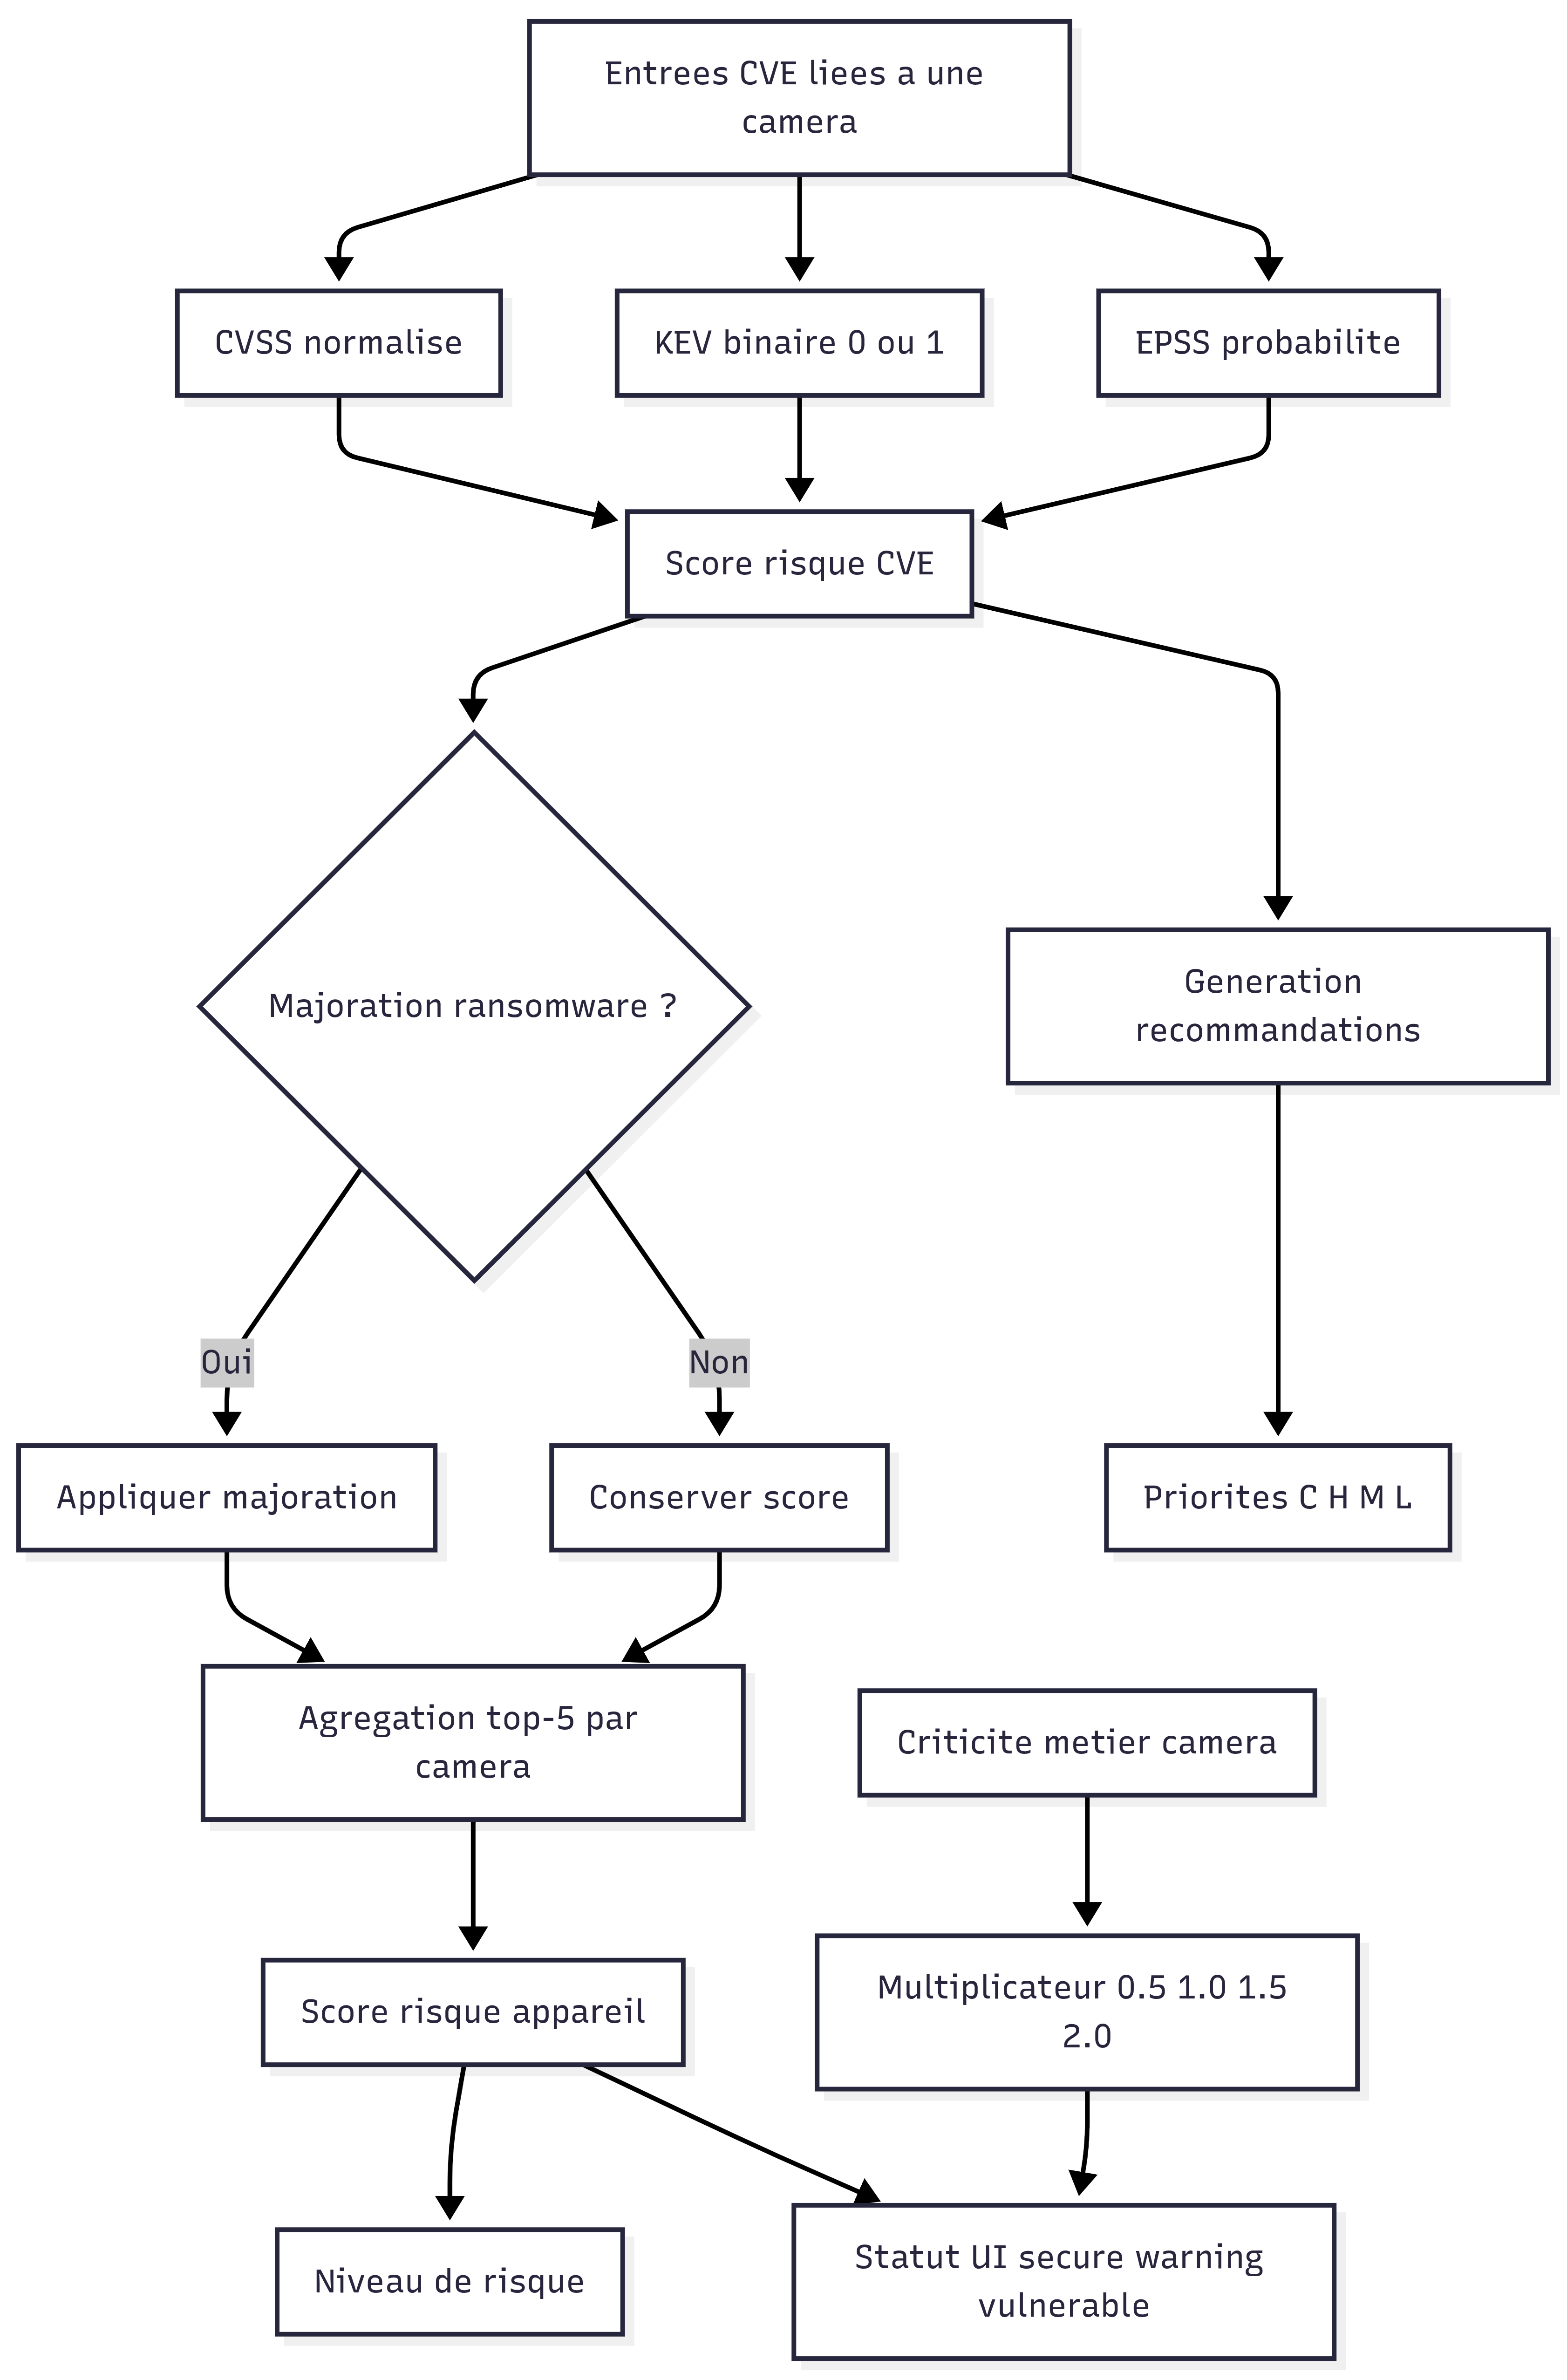
\includegraphics[width=\textwidth,height=0.72\textheight,keepaspectratio]{img/fig04-methode-priorisation-risque.png}
  \end{column}
\end{columns}
\end{frame}

\begin{frame}{Fonctionnalites de l'interface}
\begin{itemize}
  \item Gestion des cameras avec criticite metier.
  \item Analyse des menaces avec filtres (severite, source, categorie, KEV).
  \item Page detail camera: CVE, CWE, KEV, recommandations.
  \item Badges C/H/M/L: Critical, High, Medium, Low.
\end{itemize}
\end{frame}

\begin{frame}{Resultats obtenus}
\begin{itemize}
  \item Prototype operationnel de bout en bout.
  \item Execution reproductible avec Docker Compose.
  \item Donnees NVD/KEV/EPSS/CWE integrees.
  \item Priorisation plus lisible qu'une simple liste CVE.
\end{itemize}
\end{frame}

\begin{frame}{Limites et ameliorations}
\begin{itemize}
  \item Appariement vendor-produit parfois ambigu.
  \item Restitution EPSS a harmoniser dans toutes les vues.
  \item Prochaines etapes: matching, historiques, tests, exports.
  \item Extension future a d'autres familles IoT.
\end{itemize}
\end{frame}

\begin{frame}[fragile]{Demonstration et reproductibilite}
\begin{itemize}
  \item Lancement de la stack complete:
\end{itemize}
\begin{verbatim}
docker compose up --build
\end{verbatim}
\begin{itemize}
  \item Demarre Next.js, Python et PostgreSQL.
  \item Code et documentation fournis pour reproduire la demo.
\end{itemize}
\end{frame}

\begin{frame}{Conclusion}
\begin{itemize}
  \item Objectif atteint: priorisation IoT au-dela du CVSS seul.
  \item Aide concrete a la decision de remediation.
  \item Methode defensive, explicable et reproductible.
  \item Suite: industrialisation et suivi longitudinal du risque.
\end{itemize}
\end{frame}

\begin{frame}{Sources}
\footnotesize
\begin{itemize}
  \item NVD et NVD API
  \item CISA KEV Catalog
  \item FIRST EPSS et EPSS API
  \item CVE Program et CWE MITRE
  \item ETSI EN 303 645, NISTIR 8259A, NISTIR 8259B
\end{itemize}

\tiny
\url{https://nvd.nist.gov/} \quad
\url{https://www.cisa.gov/known-exploited-vulnerabilities-catalog} \quad
\url{https://www.first.org/epss/}
\end{frame}

\end{document}
